\chapter{ACTUAL WORK}
\label{ChapterActualWork}

This chapter details the actual implementation work carried out in the project, including the system architecture, TFT model implementation, training pipeline, baseline model implementation, and the ablation study design.

\section{System Architecture}

Figure \ref{fig:architecture} shows the end-to-end processing pipeline of the proposed Regime-Aware TFT (RA-TFT) framework.

\begin{figure}[h!]
\centering
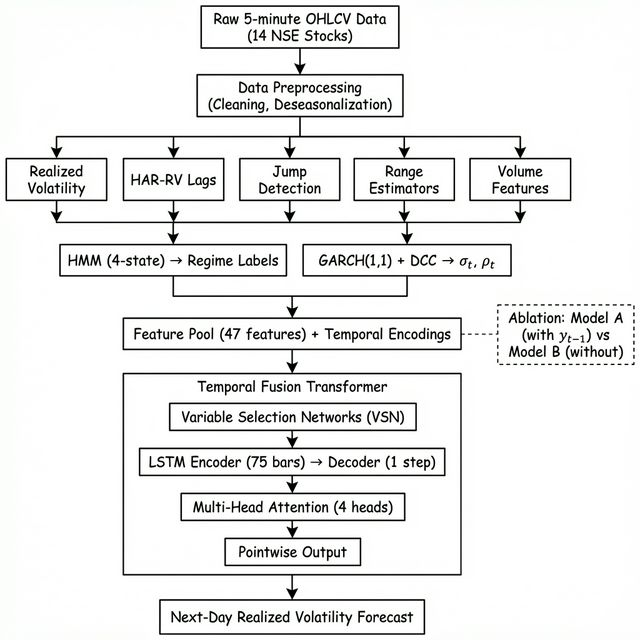
\includegraphics[width=0.85\textwidth]{Figures/system_architecture.png}
\caption{End-to-end system architecture of the Regime-Aware TFT framework}
\label{fig:architecture}
\end{figure}

The architecture comprises three main stages:

\subsection{Stage 1: Data Preprocessing}

The raw 5-minute OHLCV data for 14 stocks enters the system and undergoes preprocessing which includes outlier removal, missing value imputation, and intraday seasonality adjustment. The preprocessing pipeline is implemented in Python using pandas and NumPy, processing data stock-by-stock to maintain temporal ordering.

Key preprocessing steps include:
\begin{itemize}
    \item \textbf{Return Calculation:} Log-returns are computed as $r_t = \ln(C_t / C_{t-1})$ for each 5-minute bar.
    \item \textbf{Volume Normalization:} Trading volumes are normalized using a 20-day rolling z-score to account for cross-stock and temporal variation.
    \item \textbf{Calendar Feature Generation:} Time-of-day and day-of-week features are generated with cyclical encoding to avoid discontinuities.
\end{itemize}

\subsection{Stage 2: Feature Extraction}

Five parallel feature extraction modules compute the 47-dimensional feature vector:

\begin{enumerate}
    \item \textbf{Multi-Scale RV Module:} Computes realized volatility at four horizons (12, 38, 75, 375 bars) using vectorized NumPy operations for computational efficiency.
    \item \textbf{HAR-RV Lag Module:} Extracts lagged realized volatility values at the standard HAR offsets (1 bar, 1 hour, 1 day, 1 week).
    \item \textbf{Jump Detection Module:} Implements the Barndorff-Nielsen and Shephard bipower variation framework to separate continuous price movement from jump components.
    \item \textbf{Range Estimator Module:} Computes Parkinson, Garman-Klass, and Rogers-Satchell range-based variance estimators from OHLC data.
    \item \textbf{Volume \& Temporal Module:} Generates relative volume, volume ratio features, and cyclical temporal encodings.
\end{enumerate}

\subsection{Stage 3: Statistical Modelling Components}

Two additional components operate in parallel with the feature extraction:

\begin{enumerate}
    \item \textbf{HMM Regime Detection:} A four-state Gaussian Hidden Markov Model is fitted using the \texttt{hmmlearn} library. The model is trained on market-level daily realized volatility and log-returns. The fitted model assigns a regime label (0--3) to each trading day, which is then propagated to all intraday bars of that day.

    \item \textbf{GARCH/DCC Module:} Per-stock GARCH(1,1) models are estimated using the \texttt{arch} Python package with Student-$t$ innovations. Conditional variance estimates and standardized residuals are extracted. A DCC-inspired rolling correlation proxy is computed between each stock's returns and the equally-weighted market portfolio.
\end{enumerate}

\section{Temporal Fusion Transformer Implementation}

\subsection{Architecture Details}

The TFT architecture is implemented using the PyTorch Forecasting library built on top of PyTorch Lightning. The key architectural components are:

\begin{enumerate}
    \item \textbf{Variable Selection Networks (VSN):} Instance-specific feature weighting through softmax gates. Separate VSNs process encoder (historical) and decoder (future) inputs.

    \item \textbf{Gated Residual Networks (GRN):} Non-linear feature processing with skip connections:
    \begin{equation}
    GRN_\omega(a, c) = \text{LayerNorm}(a + \text{GLU}_\omega(\eta_1))
    \end{equation}
    where $\eta_1 = W_{1,\omega}\eta_2 + b_{1,\omega}$ and $\eta_2 = \text{ELU}(W_{2,\omega}a + W_{3,\omega}c + b_{2,\omega})$.

    \item \textbf{LSTM Encoder-Decoder:} The encoder processes 75 time-steps of historical features. The final hidden state is transferred to a one-step decoder for the prediction horizon.

    \item \textbf{Interpretable Multi-Head Attention:} Four attention heads with additive attention scoring, providing temporal attention weights that identify which historical time steps are most relevant for the prediction.
\end{enumerate}

\subsection{Model Configuration}

Table \ref{tab:config} summarizes the TFT hyperparameters selected through preliminary experimentation.

\begin{table}[h!]
\caption{TFT Model Configuration}
\label{tab:config}
\centering
\begin{tabular}{ll}
\hline
\textbf{Parameter} & \textbf{Value} \\
\hline
Total trainable parameters & 1.9M \\
Hidden size & 128 \\
Number of attention heads & 4 \\
Encoder length & 75 bars (1 day) \\
Prediction length & 1 step \\
Dropout rate & 0.15 \\
Learning rate & 0.001 \\
Early stopping patience & 15 epochs \\
Batch size & 64 \\
Batches per epoch & 1,000 \\
Target normalizer & GroupNormalizer (per-stock, softplus) \\
Loss function & RMSE \\
Learning rate scheduler & ReduceLROnPlateau \\
\hline
\end{tabular}
\end{table}

\subsection{Input Feature Organization}

The 47 features are organized into three TFT input categories:

\begin{itemize}
    \item \textbf{Static Covariates:} Stock ticker (categorical)---allows the model to learn stock-specific embeddings.
    \item \textbf{Known Future Inputs:} Calendar variables (day of week, time of day) and session flags (\texttt{is\_opening}, \texttt{is\_closing}).
    \item \textbf{Observed Past Inputs:} All volatility features (multi-scale RV, HAR lags, jump statistics, range estimators), GARCH conditional variance, DCC correlation, and HMM regime labels.
\end{itemize}

\section{Ablation Study Design}

The ablation study is central to the interpretive contribution of this project. Two model variants are trained with identical architectures but different input configurations:

\begin{itemize}
    \item \textbf{Model A (with autoregressive input):} Includes the lagged target variable $y_{t-1}$ as an observed past input. This allows the model to leverage autoregressive persistence.
    \item \textbf{Model B (without autoregressive input):} Excludes all autoregressive target inputs. The model must rely entirely on engineered features for prediction.
\end{itemize}

The critical insight motivating this design is that consecutive daily realized volatility values share 74 of 75 constituent bars (98.7\% overlap), resulting in lag-1 autocorrelation of 0.9963. The performance gap between Models A and B directly quantifies how much predictive power derives from autoregressive memory versus genuine feature-based information.

\section{Baseline Model Implementation}

\subsection{HAR-RV Implementation}

The Heterogeneous Autoregressive model of Realized Volatility \cite{corsi2009} is implemented using ordinary least squares (OLS) regression with Newey-West standard errors to account for serial correlation:

\begin{equation}
RV_{t+1}^{(d)} = \beta_0 + \beta_d RV_t^{(d)} + \beta_w RV_t^{(w)} + \beta_m RV_t^{(m)} + \epsilon_t
\end{equation}

where $RV^{(d)}$, $RV^{(w)}$, and $RV^{(m)}$ denote daily, weekly, and monthly realized volatility respectively. The model is fitted separately for each stock using the \texttt{statsmodels} library.

\subsection{GARCH Family Implementation}

Three GARCH variants are implemented using the \texttt{arch} Python package:

\begin{enumerate}
    \item \textbf{GARCH(1,1):} Standard symmetric GARCH with Student-$t$ innovations.
    \item \textbf{EGARCH(1,1):} Exponential GARCH capturing asymmetric effects.
    \item \textbf{GJR-GARCH(1,1):} Threshold GARCH with explicit leverage indicator.
\end{enumerate}

For each stock, all three variants are fitted and the best model is selected by Akaike Information Criterion (AIC). Out-of-sample forecasts are generated using rolling one-step-ahead predictions.

\section{Training Pipeline}

The training pipeline is implemented on Kaggle's GPU infrastructure (NVIDIA T4/P100) using PyTorch Lightning:

\begin{enumerate}
    \item \textbf{Data Loading:} The PyTorch Forecasting \texttt{TimeSeriesDataSet} handles time-windowing, feature scaling, and batch construction.
    \item \textbf{Training Loop:} RMSE loss is minimized using the Adam optimizer with an initial learning rate of 0.001. The \texttt{ReduceLROnPlateau} scheduler reduces the learning rate by a factor of 0.5 after 5 epochs without validation improvement.
    \item \textbf{Early Stopping:} Training halts after 15 consecutive epochs without validation loss improvement.
    \item \textbf{Checkpointing:} The best model state (by validation loss) is saved and used for final evaluation.
\end{enumerate}

\section{Implementation Tools and Technologies}

Table \ref{tab:tools} summarizes the key tools and libraries used in this project.

\begin{table}[h!]
\caption{Tools and Technologies Used}
\label{tab:tools}
\centering
\begin{tabular}{ll}
\hline
\textbf{Component} & \textbf{Tool/Library} \\
\hline
Programming Language & Python 3.10 \\
Deep Learning Framework & PyTorch 2.1 \\
TFT Implementation & PyTorch Forecasting \\
Training Infrastructure & PyTorch Lightning \\
GARCH Models & \texttt{arch} package \\
HMM Implementation & \texttt{hmmlearn} \\
Data Processing & pandas, NumPy \\
Statistical Analysis & statsmodels, scipy \\
Visualization & matplotlib, seaborn \\
Compute Platform & Kaggle (NVIDIA T4/P100 GPU) \\
\hline
\end{tabular}
\end{table}
